\documentclass[11pt]{article}
\usepackage[margin=1in]{geometry}
\usepackage{booktabs}
\usepackage{array}
\usepackage[table]{xcolor}
\definecolor{morblue}{RGB}{218,232,252}
\usepackage{caption}
\usepackage{amsmath}
\usepackage{helvet}
\usepackage{tikz}
\usetikzlibrary{arrows.meta, positioning, shapes.geometric}
\renewcommand{\familydefault}{\sfdefault}

\newcolumntype{R}{>{\raggedleft\arraybackslash}p{1.7cm}}
\captionsetup{font=small, labelfont=bf}

\newcommand{\best}[1]{\textbf{#1}}

\title{\vspace{-2.5em}Recursive Genomic Q-Former:\\ Parameter-Reduction vs.\ Performance Trade-off}
\author{}
\date{}

\begin{document}
\maketitle
\vspace{-3em}

\begin{center}
\setlength{\fboxsep}{10pt}
\fcolorbox{black!40}{black!4}{%
\begin{minipage}{0.94\textwidth}
\textbf{\large Task details}\\[0.4em]
\begin{tabular}{@{}p{3.1cm}p{\dimexpr\textwidth-3.6cm}@{}}
\textbf{Task} & \texttt{cancer\_type} --- 4-way tumor-of-origin classification from bulk
gene-expression profiles (TCGA RNA-seq). \\[0.3em]
\textbf{Dataset} & Unified TCGA cohort: 2{,}738 samples $\times$ 20{,}530 genes; top
4{,}000 highly-variable genes used as input tokens. \\[0.3em]
\textbf{Classes} & Breast (BRCA, 867), Head--neck (HNSC, 423), Lung (LUNG, 943),
Prostate (PRAD, 505). \\[0.3em]
\textbf{Split} & 70/15/15 train/val/test, \textbf{523 test samples}, seed 42. \\[0.3em]
\textbf{Model} & Recursive Genomic Q-Former: $d_{\text{model}}=128$, 256 marker query
slots, recursion depth 4. \\[0.3em]
\textbf{Metric} & Test accuracy and macro-averaged F1. \\
\end{tabular}
\end{minipage}}
\end{center}
\vspace{0.4em}

%---------------------------------------------------------------
\begin{center}
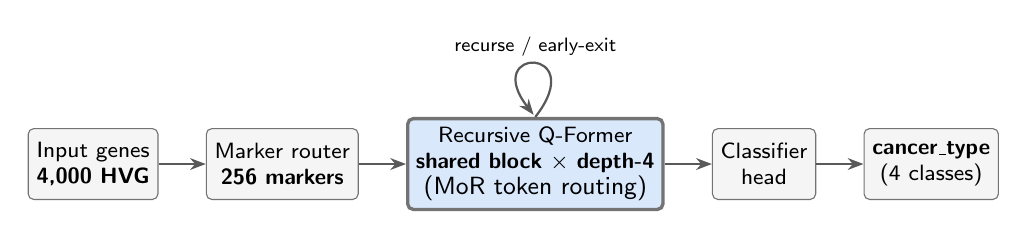
\begin{tikzpicture}[
  node distance=6mm,
  font=\footnotesize,
  box/.style={rectangle, rounded corners=2pt, draw=black!55, fill=black!4,
              minimum height=9mm, align=center, inner sep=3pt},
  mor/.style={rectangle, rounded corners=2pt, draw=black!55, fill=morblue,
              very thick, minimum height=9mm, align=center, inner sep=3pt},
  arr/.style={-{Stealth[length=2mm]}, thick, draw=black!65}
]
\node[box] (in) {Input genes\\\textbf{4{,}000 HVG}};
\node[box, right=of in] (mark) {Marker router\\\textbf{256 markers}};
\node[mor, right=of mark] (rec) {Recursive Q-Former\\\textbf{shared block $\times$ depth-4}\\\small(MoR token routing)};
\node[box, right=of rec] (head) {Classifier\\head};
\node[box, right=of head] (out) {\textbf{cancer\_type}\\(4 classes)};

\draw[arr] (in) -- (mark);
\draw[arr] (mark) -- (rec);
\draw[arr] (rec) -- (head);
\draw[arr] (head) -- (out);

% recursion self-loop on the shared block
\draw[arr, shorten >=1pt] (rec.north) .. controls +(0.7,0.9) and +(-0.7,0.9) .. (rec.north)
  node[midway, above, yshift=-1pt] {\scriptsize recurse / early-exit};
\end{tikzpicture}

\textit{\footnotesize Figure 1: Pipeline. The shared transformer block (blue) is reused
across recursion steps; MoR routes tokens to a per-token depth instead of a fixed pass.}
\end{center}
\vspace{0.6em}

\noindent
All results are on the \textbf{cancer\_type} classification head (4 classes: BRCA, HNSC,
LUNG, PRAD; 523 test samples), with a fixed recursion depth of 4, $d_{\text{model}}=128$,
256 marker query slots, and seed 42. The ``regular'' recursive model shares one
transformer block across all recursion steps; the comparison models either un-tie those
weights (\emph{Independent}) or add token-adaptive routing (\emph{MoR}).

%---------------------------------------------------------------
\begin{table}[h]
\centering
\caption{\textbf{Main parameter-reduction trade-off.} Sharing the transformer block across
the 4 recursion steps cuts transformer parameters by $\sim$4$\times$ versus an
un-shared (independent) stack, while losing only 0.57 accuracy points. Mixture-of-Recursions
(MoR) token routing keeps the shared (small) parameter count yet recovers most of the gap and
saves $\sim$41\% compute.}
\label{tab:main}
\begin{tabular}{l l c r c r r}
\toprule
\textbf{Model} & \textbf{Weights} & \textbf{Routing} &
\textbf{Transf.\ params} & \textbf{Param} &
\textbf{Test acc.} & \textbf{Macro-F1} \\
 & & & & \textbf{ratio} & & \\
\midrule
Independent stack       & untied  & none           & 530{,}432 & 3.99$\times$ & \best{0.9904} & 0.9891 \\
\textbf{Recursive (shared)} & shared  & none       & 132{,}992 & 1.00$\times$ & 0.9847 & 0.9871 \\
\rowcolor{morblue} \textbf{MoR (token-adaptive)} & \textbf{shared} & \textbf{token} & \textbf{132{,}992} & \textbf{1.00$\times$} & \best{0.9885} & \best{0.9892} \\
\bottomrule
\end{tabular}
\end{table}

\noindent
\textbf{Read-out.} The shared recursive model uses \textbf{74.9\% fewer} transformer
parameters than the independent stack (132{,}992 vs.\ 530{,}432) for a \textbf{0.57-point}
accuracy cost. Adding MoR token routing closes that gap to \textbf{0.19 points} at the same
small parameter budget, and is the only configuration that also reduces FLOPs.

\vspace{1em}
%---------------------------------------------------------------
\begin{table}[h]
\centering
\caption{\textbf{Parameter scaling vs.\ recursion depth.} Shared-weight recursion keeps the
transformer parameter count essentially flat as depth grows, whereas an independent stack
grows linearly. The reduction factor reaches nearly 8$\times$ at depth 8.}
\label{tab:scaling}
\begin{tabular}{c r r c}
\toprule
\textbf{Recursion depth} & \textbf{Shared params} & \textbf{Independent params} &
\textbf{Reduction factor} \\
\midrule
1 & 132{,}608 & 132{,}608   & 1.00$\times$ \\
2 & 132{,}736 & 265{,}216   & 2.00$\times$ \\
4 & 132{,}992 & 530{,}432   & 3.99$\times$ \\
6 & 133{,}248 & 795{,}648   & 5.97$\times$ \\
8 & 133{,}504 & 1{,}060{,}864 & 7.95$\times$ \\
\bottomrule
\end{tabular}
\end{table}

\vspace{1em}
%---------------------------------------------------------------
\begin{table}[h]
\centering
\caption{\textbf{Compute trade-off (depth-4 variants).} Early-exit / adaptive recursion lowers
the \emph{effective} mean depth and FLOPs per sample relative to a fixed depth-4 pass, at equal
parameter count. MoR achieves the lowest compute and the best F1.}
\label{tab:compute}
\begin{tabular}{l r r r r}
\toprule
\textbf{Configuration} & \textbf{Transf.\ params} & \textbf{Mean depth} &
\textbf{MFLOPs/sample} & \textbf{Test acc.} \\
\midrule
Fixed depth-4 (no early exit)   & 132{,}480 & 4.00 & 268.4 & 0.9847 \\
Recursive (shared, early-exit)  & 132{,}992 & 2.75 & 161.5 & 0.9847 \\
No recursive refine             & 132{,}992 & 2.75 & 161.5 & 0.9771 \\
\rowcolor{morblue} \textbf{MoR (token-adaptive)} & \textbf{132{,}992} & \textbf{2.69} & \best{159.1} & \best{0.9885} \\
\bottomrule
\end{tabular}
\end{table}

\vspace{0.5em}
\noindent\footnotesize
\textit{Notes.} Param ratio in Table~\ref{tab:main} is independent$/$shared transformer
parameters. ``Transf.\ params'' counts only the recurrent transformer block (the full model
incl.\ embeddings/heads is $\sim$712K for shared variants, $\sim$1.11M for the independent
stack). Compute-saving for the early-exit and MoR variants is $\approx$40\% of the fixed
depth-4 FLOP budget. Token-reduction at the marker stage additionally compresses 4000 input
genes to 256 retained markers (93.6\% token reduction) at 98.5\% accuracy.

\end{document}
